% !TeX program = LuaLaTeX

\documentclass{tufte-handout}

%\geometry{showframe}% for debugging purposes -- displays the margins

\usepackage{amsmath}

% Set up the images/graphics package
\usepackage{graphicx}
\setkeys{Gin}{width=\linewidth,totalheight=\textheight,keepaspectratio}
\graphicspath{{graphics/}}
\DeclareGraphicsExtensions{.pdf,.png,.jpg}


\usepackage{tabularx}

\usepackage{fancyvrb}

% NLS --------

\usepackage[spanish]{babel}
\usepackage[latin1]{inputenc}
\selectlanguage{spanish}

%\usepackage{fontspec}
%\usepackage[T1]{fontenc}

%\usepackage{uarial}

%%\newfontfamily\fntarialbold{A030-Bol}
%\newfontfamily\fntarialregular{A030-Reg}

%\newcommand{\aaf}{\fntarialregular actio\textcolor{red}{ad}futurum }
\newcommand{\aaf}{{\sf actio \textcolor{red}{ad} futurum }}

% The following package makes prettier tables.  We're all about the bling!
\usepackage{booktabs}

% The units package provides nice, non-stacked fractions and better spacing
% for units.
\usepackage{units}

% The fancyvrb package lets us customize the formatting of verbatim
% environments.  We use a slightly smaller font.
\usepackage{fancyvrb}
\fvset{fontsize=\normalsize}

% Small sections of multiple columns
\usepackage{multicol}

% Provides paragraphs of dummy text
\usepackage{lipsum}

% These commands are used to pretty-print LaTeX commands
\newcommand{\doccmd}[1]{\texttt{\textbackslash#1}}% command name -- adds backslash automatically
\newcommand{\docopt}[1]{\ensuremath{\langle}\textrm{\textit{#1}}\ensuremath{\rangle}}% optional command argument
\newcommand{\docarg}[1]{\textrm{\textit{#1}}}% (required) command argument
\newenvironment{docspec}{\begin{quote}\noindent}{\end{quote}}% command specification environment
\newcommand{\docenv}[1]{\textsf{#1}}% environment name
\newcommand{\docpkg}[1]{\texttt{#1}}% package name
\newcommand{\doccls}[1]{\texttt{#1}}% document class name
\newcommand{\docclsopt}[1]{\texttt{#1}}% document class option name


\newcommand{\ifb}{\texttt{Intranet-firebug}}% 
\newcommand{\aaa}[1]{\textsf{#1}}% test
\newcommand{\fireBug}{\textbf{\textsf{firebug}}}% 
\newcommand{\FirebugLite}{\hbox{\textbf{\textsf{fireBugLite}}}}%
\newcommand{\Firebug}{\textsc{Firebug}}% 
\newcommand{\Firefox}{\textsc{Firefox}}% 
\newcommand{\FirePHP}{\textsc{FirePHP}}% 
\newcommand{\Sourceforge}{\textsc{Sourceforge}}% 
\newcommand{\TCL}{\textbf{TCL}}% 
\newcommand{\ADP}{\textbf{ADP}}% 

\newcommand{\PostgresSQL}{\textbf{PostgresSQL}}% 
\newcommand{\OpenACS}{\textbf{OpenACS}}%
\newcommand{\HTML}{\textbf{HTML}}%
\newcommand{\DOM}{\textbf{DOM}}%
\newcommand{\AJAX}{\textbf{AJAX}}%
\newcommand{\CSS}{\textbf{AJAX}}%
\newcommand{\API}{\textbf{API}}%
\newcommand{\api}[1]{\texttt{#1}}% 
\newcommand{\HTTP}{\textbf{HTTP}}%
\newcommand{\Wildfire}{\textsc{Wildfire}}%

\newcommand{\chrome}{\textbf{Chrome}}
\newcommand{\FirePHPForChrome}{\hbox{\textbf{FirePHP4Chrome}}}

\newcommand{\ie}{\textbf{Internet Explorer}}

\newcommand{\po}{{\sf \textcolor{blue}{]}Project-Open\textcolor{blue}{[}}}%
\newcommand{\jvaemail}{jv@actioadfuturum.com}
\newcommand{\opsrc}{"Open~Source"} %

\newenvironment{mylist}[1]%
  {\begin{list}{}{\settowidth{\labelwidth}{\textbf{#1}}
   \setlength{\leftmargin}{\labelwidth}
   \addtolength{\leftmargin}{\labelsep}
   \renewcommand{\makelabel}[1]{\textbf{\hfill##1}}}}%
  {\end{list}}


 % Set up the spacing using fontspec features
 % \renewcommand\allcapsspacing[1]{{\addfontfeature{LetterSpace=15}#1}}
 % \renewcommand\smallcapsspacing[1]{{\addfontfeature{LetterSpace=10}#1}}

% -------------
\title{intranet-firebug - Una adaptación del API de \mbox{FirePHP} en \mbox{TCL} para facilitar la depuración de desarrollos \mbox{sobre} \po  }
\author[Josep Vela]{Josep Vela - \textsf{ \aaf\ }  - \texttt{\jvaemail}}
\date{Versión 0.3 - Marzo 2012}

\begin{document}

\maketitle% this prints the handout title, author, and date

\begin{abstract}

\noindent Este documento describe el paquete \ifb\ implementación de \FirePHP\ en \TCL. El documento proporciona ejemplos de uso e imágenes de la captura del resultado de la ejecución de los ejemplos en la consola de \Firebug. \sidenote{La motivación original en el desarrollo del paquete se debe al proceso de aprendizaje de \po }
\end{abstract}

\section{Descripción}\label{sec:descr}
\OpenACS\ \sidenote{\url{www.openacs.org}}  es un entorno  \opsrc\ de desarrollo de aplicaciones web que actualmente está presente en muchos productos y sitios Web y en particular en entornos de aprendizaje y de gestión de proyectos. Los orígenes de \OpenACS\ se remontan al año 1995, siendo al final del 2000 cuando se termina la integración con la base de datos \PostgresSQL\ \sidenote{\url{www.postgresql.org}}  y se licencia bajo  \opsrc\ . Desde su inicio \TCL\ es el lenguaje usado para la programación de los scripts en \OpenACS, en parte por su sencillez y en parte por la integración con los conceptos multitarea que facilitan disponer de un servidor Web completo y robusto. La integración en \OpenACS\ con \TCL\ \sidenote{\url{www.tcl.tk}} y la Base de Datos proporciona un servidor que dispone de un conjunto importante de facilidades de desarrollo de aplicaciones. Sin embargo los mecanismos de depuración son los clásicos y no facilitan el desarrollo de las nuevas aplicaciones basadas en \AJAX\ \sidenote{\url{www.w3schools.com/ajax/default.asp}} ni sacan provecho de los avances en la depuración proporcionados por los navegadores. 

\Firebug\ \sidenote{\url{www.firephp.org}} es por otra parte la herramienta de ayuda al desarrollo Web muy popular que permite el análisis y la modificación del  \HTML\ que recibe el navegador, tanto directamente como por medio de la manipulación del \DOM\ incluyendo tanto JavaScript como \CSS. \Firebug\ facilita además  la inspección del uso de la red y del rendimiento que produce la carga de las páginas. \Firebug\ era originariamente un desarrollo para \Firefox, pero actualmente está disponible para otros navegadores en una modalidad “Lite”. \Firebug\ dispone además de facilidades para desarrollar extensiones con lo que permite dotarlo de mayor potencia. 
\newpage
\section{El paquete \ifb\ }

El paquete \ifb\ se plantea como una facilidad de ayuda al desarrollo de nuevas funcionalidades sobre el entorno \po\sidenote{\url{www.project-open.com}}. 

\po\ es una solución \opsrc\ de gestión de proyectos bajo un punto de vista de control financiero y de gestión muy completo y altamente parametrizable. Al estar desarrollado sobre \OpenACS\ hace un uso intensivo de las facilidades disponibles y añade toda una serie de paquetes \TCL\ que ofrecen las funcionalidades extras de la gestión de proyectos.

 \po\ dispone de una vasta documentación del modelo de objetos que implementa sobre \PostgresSQL\ y de los paquetes desarrollados, así como de una comunidad activa y creciente en \Sourceforge\ \sidenote{\url{www.sourceforge.net}}. Sin embargo a la hora de realizar la inmersión dentro de \po, es necesario disponer del máximo de información sobre el flujo de las páginas y en muchos casos sin que está información penalice la representación de la pantalla final en el navegador.
Mediante los mecanismos habituales de depuración disponibles en \OpenACS, puede obtenerse una traza en ficheros de log usando la \API\ \sidenote{Aplication Program Interface} \api{ns\_log} y a continuación usar las facilidades del sistema operativo para buscar la información (\api{cat}, \api{tail}, \api{grep})\sidenote{Instrucciones UNIX}.  Además de estos mecanismos, \OpenACS\ dispone de la variable de configuración \api{debug} que si se activa produce gran cantidad de información de ayuda a la depuración.
Otro mecanismo habitual consiste en añadir texto adicional de depuración en la página \HTML\ insertado como contenido. Este mecanismo que si bien facilita el mostrar los datos, casi siempre acaba corrompiendo el formato de presentación con lo que en muchos casos no es aconsejable.

Bajo estos conceptos se desarrolla \Firebug\ que usando cabeceras adicionales dentro del protocolo \HTTP\ permite el enviar datos de depuración al navegador. Estos datos no se muestran en las páginas  \HTML\ puesto que forman parte de las cabeceras del protocolo y si se dispone de un añadido en el navegador que permita mostrar estas cabeceras de forma que no afecte la presentación de la pagina se consigue un mecanismo no intrusivo de trazabilidad de datos de depuración. Por lo tanto \Firebug\ consta de una extensión que se instala en el navegador y de unas librerías que se utilizan en el servidor para añadir la información de depuración en las cabeceras del protocolo \HTTP. Estas cabeceras forman la extensión del protocolo conocido como \Wildfire\sidenote{\url{www.wildfirehq.org}} e implantado siguiendo los conceptos aplicados en el núcleo de la librería \FirePHP.
El paquete \ifb\ proporciona una implantación similar a la librería \FirePHP\ pero usando \TCL\ para la integración en las paginas generadas por \OpenACS.

Las facilidades de depuración están disponibles originalmente para \Firefox\ pero existen añadidos para \chrome\ gracias a \FirePHPForChrome\ desarrollado por Aaron Saray  \sidenote{\url{https://github.com/aaronsaray/FirePHP4Chrome}} y para \ie\ usando \FirebugLite .

\section{Descripción}
\fireBug\  - Muestra información de depuración en la consola del navegador
\subsection{Formato}
\fireBug\ mensaje  ¿arg arg? 

%\begin{tikzpicture}
%%\path [fill=yellow] (0,0) -- (0,5) to [out=-80, in=160]
%(3,.8) -- (3,0) -- (0,0);
%\draw [<->] (0,6) node [left] {$P$} -- (0,0)
%node [below left] {(0,0)} -- (7,0) node [below] {$Q$};
%\draw [ultra thick, dashed] (0,.8) node [left] {$P^*=.8$} -- (3,.8)
%-- (3,0) node [below] {$Q^*=3$};
%\draw [fill] (3,.8) circle [radius=.1];
%\draw [thick] (0,5) to [out=-80, in=160] (3,.8) to
%[out=-20, in=175] (6,0);
%\end{tikzpicture}



\subsection{Opciones}
\begin{table}[ht]
 % \centering
  \fontfamily{ppl}\selectfont
  \begin{tabularx}{0.80\textwidth}{lX}
%    \toprule
%    Parametro & Descripción \\
%    \midrule
-type & Tipo de mensaje que se representa por un icono distinto. \\
& Los parametros permitidos son:\\
& \texttt{LOG}, \texttt{WARN}, \texttt{INFO}, \texttt{ERROR}. \\ 
& Por defecto es \texttt{LOG}. \\
-collapsed &  Muestra un grupo de mensajes sin desplegar.\\
-color & Destaca los mensajes en un color distintivo.\\
-label & Permite añadir una etiqueta identificativa.\\
-group & Permite agrupar los mensajes. \\
-output & El mensaje a mostrar en la consola.\\ 
%    \bottomrule
  \end{tabularx}
  \caption{Parametros de la función }
  \label{tab:params}
\end{table}

\subsection{Funciones auxiliares}

De cara a simplificar el uso de las funciones de depuración se han creado las siguientes funciones:
\begin{table}[ht]
  %\centering
  \fontfamily{ppl}\selectfont
  \begin{tabularx}{\textwidth}{lX}
	\texttt{fb\_log   mensaje} &– Muestra un mensaje simple de log.\\
\texttt{fb\_warn  mensaje} &– Muestra un mensaje con un icono de peligro. \\
\texttt{fb\_info  mensaje} &– Muestra un mensaje con un icono de información. \\
\texttt{fb\_error mensaje} &– Muestra un mensaje con un icono de error \\
\texttt{fb\_var  \$varname} &– Muestra el valor de la variable indicada \\
  \end{tabularx}
  \caption{Funciones auxiliares}
  \label{tab:auxfuncs}
\end{table}

\newpage
\subsection{Ejemplos}
%\enlargethispage{1cm}
El código \TCL\ siguiente muestra un ejemplo simple de \mbox{\it timestamp} cuyo resultado de ejecución conjuntamente con el código de la plantilla \ADP\ se muestra en las figuras 1, 2, 3 y que corresponden a la captura de la pagina del navegador \Firefox, y a la consola de \Firebug.

\begin{Verbatim}[fontsize=\footnotesize,frame=lines,label=Código Fuente: test-fb.tcl,labelposition=topline,numbers=left,stepnumber=1,samepage=true]

# ----------------------------------------------------------------------
#
# test-fb.tcl 
#
#    @author        Josep Vela - jv@actioadfuturum.com
#    @creation-date $Date$
#    @cvs-id        $Id$
#
# ----------------------------------------------------------------------

set tt [format "The time is now => %s" [clock format [clock seconds] -format %H:%M:%S] ]

fireBug $tt -label "A timestamp sample"

fb_log    $tt 

fb_log    "Plain_Message" 
fb_info   "Info_Message" 
fb_warn   "Warn_Message"
fb_error  "Error_Message"

set aa {a {1 2 3} b {4 5}}
fb_var $aa

set bb {i 10 j 20}
fb_var $bb

fireBug "" -label "Group ID as Label" -group begin -collapsed false 
fireBug "Inside_the_group_1" -type INFO 
fireBug "Inside_the_group_2" -type WARN
fireBug "" -group end 

fireBug "Group ID as Message" -group begin -collapsed true -color "#FF00FF"
for { set i 1 } { $i <= 10 } { incr i } { fireBug "test $i" }
fireBug "" -group end

set aTable { {"Col 1 Heading" "Col 2 Heading"} 
             {"Row 1 Col 1" "Row 1 Col 2" } 
             {"Row 2 Col 1" "Row 2 Col 2" } 
             {"Row 3 Col 1" "Row 3 Col 2" } }

fireBug $aTable -label "Table label" -type TABLE
fireBug $aTable -type TABLE

# ----------------------------------------------------------------------
#   $Log$
# ----------------------------------------------------------------------

\end{Verbatim}

\newpage
\begin{Verbatim}[fontsize=\footnotesize,frame=lines,label=Código Fuente Plantilla: test-fb.adp,labelposition=topline,numbers=left,stepnumber=1,samepage=true]

<!--------------------------------------------------------------------- 

 test-fb.adp 

   @author        Josep Vela - jv@actioadfuturum.com
   @creation-date $Date$
   @cvs-id        $Id$

----------------------------------------------------------------------->
<h1>Sample FireBug interface for TCL</h1>
<h2>@tt@</h2>

\end{Verbatim}


%\begin{marginfigure}%
%  \includegraphics[width=\linewidth]{helix}
%  \caption{caption \url{http://asymptote.sf.net/}}
%  \label{fig:marginfig}
%\end{marginfigure}

%\begin{figure*}[h]
%  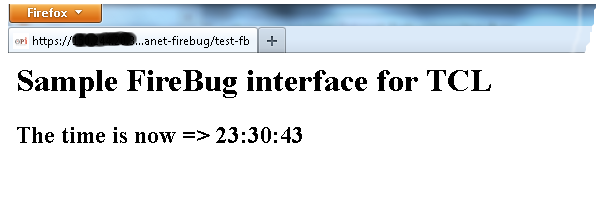
\includegraphics[width=\linewidth]{fb-01.png}%
%  \caption{La figura muestra una captura completa del navegador Firefox}%
%  \label{fig:fullfig1}%
%\end{figure*}

%Torn Paper Effect using GIMP, http://www.pixeldigest.com/ripped_paper.html

A continuación vemos el resultado de la ejecución del \emph{script} de \TCL\ y su correspondiente \emph{Template} de presentación \ADP.
\begin{figure}
  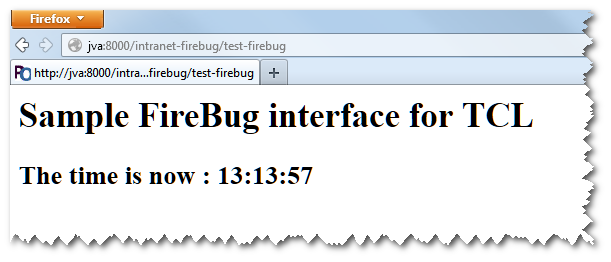
\includegraphics{fb-01-ok.png}%
  \caption{La figura muestra una captura del navegador \Firefox\ con el resultado de la ejecución del \TCL\ de ejemplo}%
  \label{fig:ff-html}%
  \setfloatalignment{b}
\end{figure}

La figura siguiente muestra el resultado de la ejecución de correspondientes a las lineas
14, 16, 18--21, 24 27 y siguientes del código \TCL. 
\begin{figure}
  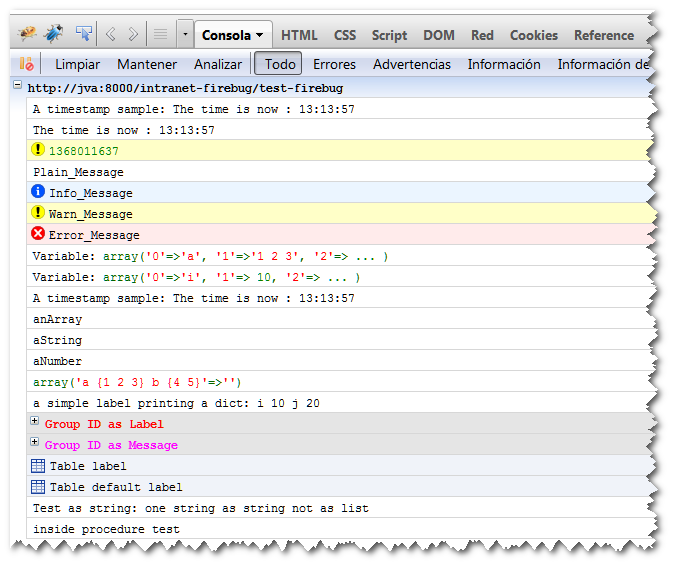
\includegraphics{fb-02-ok-ok.png}%
  \caption{La figura muestra una captura del navegador \Firefox\ con la consola de \Firebug\ activada}%
  \label{fig:ff-consola}%
  \setfloatalignment{b}
\end{figure}

La figura siguiente muestra en la consola \Firebug el resultado de la ejecución correspondientes a las lineas 34, 43 y 44, una vez expandidos los diversos grupos y la primera tabla.

\begin{figure}
  %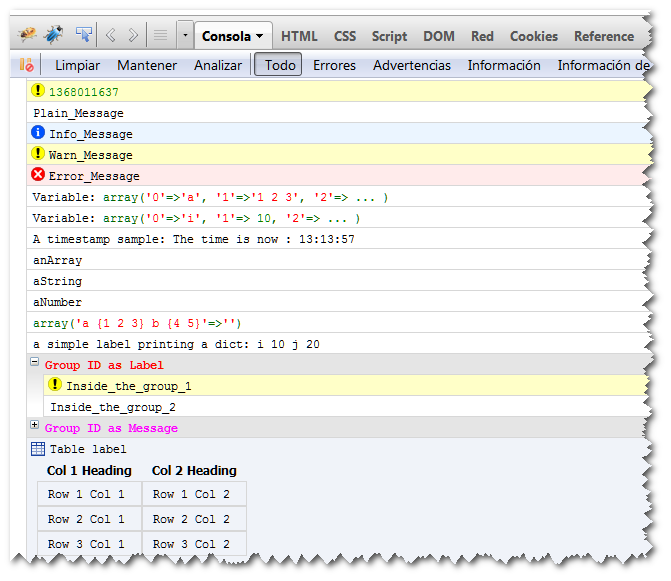
\includegraphics[width=0.50\linewidth]{fb-03-ok-ok.png}%
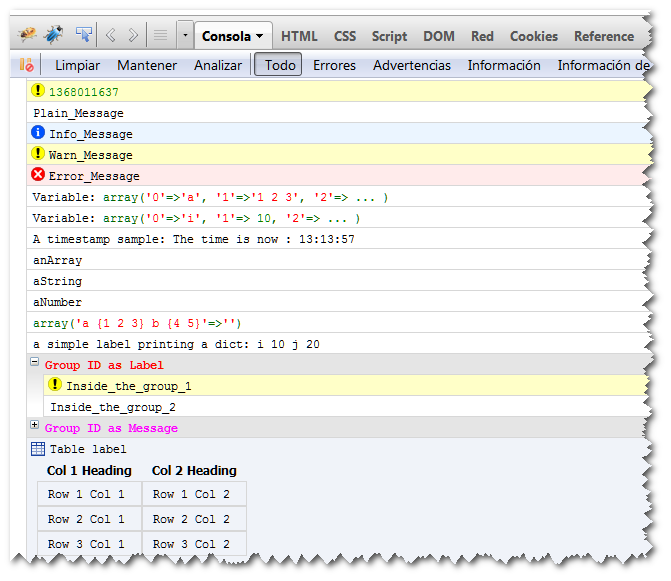
\includegraphics{fb-03-ok-ok.png}%
  \caption{Consola de \Firebug con el tipo \textbf{Grupo} expandido y la primera \textbf{Tabla} también expandida.}%
  \label{fig:ff-consola-detalle}%
  \setfloatalignment{b}
\end{figure}

\section{Documentación auxiliar}
Para documentación auxiliar ver los enlaces referidos en las notas al margen

\section{Soporte}\label{sec:support}
Cualquier consulta sobre el paquete puede realizarse a la dirección de correo electrónico 
\texttt{\jvaemail} indicada o en la página web de \url{http://www.actioadfuturum.com}.

%\bibliography{sample-handout}
%\bibliographystyle{plainnat}


\end{document}
